\subsection{Background}

The Micro Flapping Wing Flyer uses a flexible membrane wing, and the way this wing changes shape during motion plays a major role in how it behaves aerodynamically. Static testing alone cannot show this because the wing does not stay rigid when it flaps. Instead, it bends, lags, twists slightly, and responds to the forces acting on it. These dynamic effects are known to influence lift and overall performance, which has been shown in previous flapping wing research such as Lentink and Dickinson~\cite{Lentink2009}.

Since the previous capstone team already completed detailed static testing for the same wing geometries used this year, repeating that work during this semester would not have added new information. Because of this, my focus was on building the dynamic testing capability: creating a setup that allowed the wing to be flapped while being recorded clearly, and developing a MATLAB system that could track how the wing deformed throughout motion. This dynamic behaviour is needed so that we can eventually compare wings not just by stiffness, but by how they behave when actually moving. A calibration step was also introduced so the pixel motion could be converted into millimetres, allowing the deformation results to be expressed in physical units.
 
\subsection{Dynamic Testing Setup}

At the start of the semester, I tested several different ways to record the wing. The biggest issue early on was getting clean footage that the tracking algorithm could work with. The membrane surface reflects light easily, so small changes in angle or lighting caused glare or shadows that made the markers hard to detect. Some backgrounds blended with the wing, and different camera heights caused distortion.

After multiple trials with different lighting, backgrounds, and phone positions, the setup that worked best used an overhead camera looking straight down onto a white background. The white surface removed most of the clutter and shadows and made the markers stand out clearly. The top-down view also ensured that the wing appeared as a clean 2D projection, which is important since the tracking script measures pixel displacement frame by frame. This layout was stable and gave the most consistent detection results throughout the semester. This setup is now fully repeatable for all future wing prototypes and will be used as the standard configuration for the dynamic database.
 
\begin{figure}[htb]

    \centering

    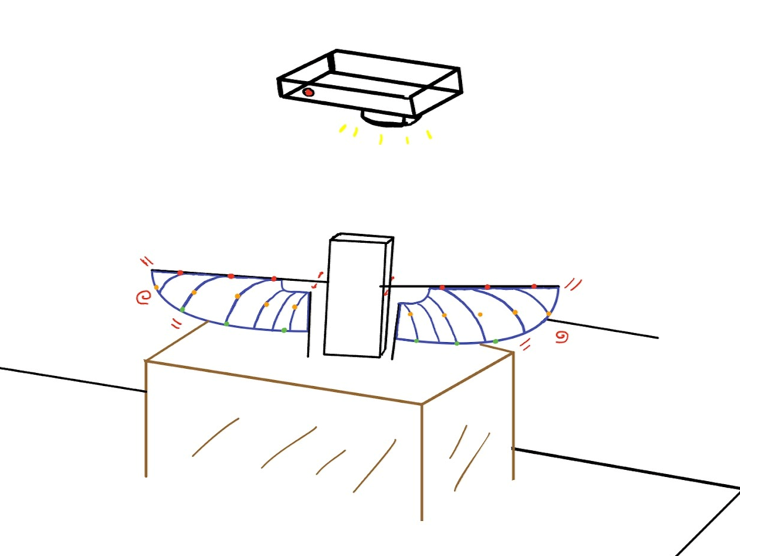
\includegraphics[height = 6.5cm]{figures/Dynamic Testing Setup.png}

    \caption{Dynamic Test Setup}

    \label{fig:dynamic_setup}

\end{figure}
 
\subsection{Marker Placement}
To measure how the wing bends while flapping, I applied three coloured markers along the span. A green marker was placed at the root, a red marker at the mid span rib, and a blue marker at the wing tip. These points were selected because they represent three key structural locations. The root gives information on how much the mount shifts or flexes, the mid span shows how the membrane bends during motion, and the tip experiences the greatest displacement.

This style of marker placement is also used in insect wing studies where researchers track a few points to understand bending patterns~\cite{Bomphrey2010}.
 
\begin{figure}[htb]

    \centering

    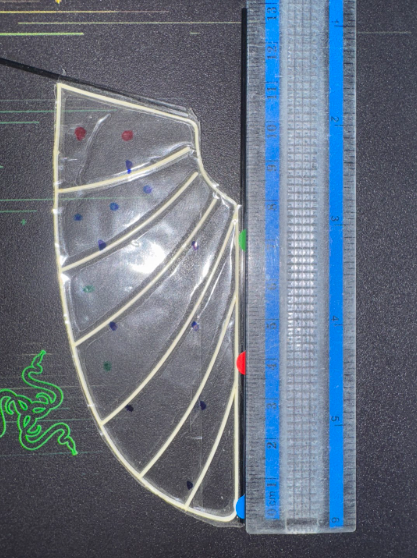
\includegraphics[height = 6.5cm]{figures/Wing w Test Markers.png}

    \caption{Wing with Marker Placement.}

    \label{fig:marker_placement}

\end{figure}
 
\subsection{Motion Tracking Development}

With the physical setup established, the next objective was to develop a MATLAB-based tracking pipeline. Each recorded video was processed frame by frame, converted from RGB to HSV colour space, and segmented using tuned thresholds for each marker colour. HSV segmentation was chosen because it is better to ambient lighting variation, improving detection consistency. For every frame, the centroid of each detected colour region was extracted. Missing detections were interpolated and small frame-to-frame jitter was smoothed to produce continuous trajectories.
 
Beyond producing numerical outputs, the system generated an overlay video displaying the original footage with tracked marker positions and their motion paths superimposed. This provided immediate visual confirmation that the segmentation and tracking were functioning correctly. If the overlay accurately matched the motion of the physical markers, the extracted data was considered valid. Figure~\ref{fig:tracking_overlay} shows an example frame from one of these overlay videos.
 
\begin{figure}[htb]

    \centering

    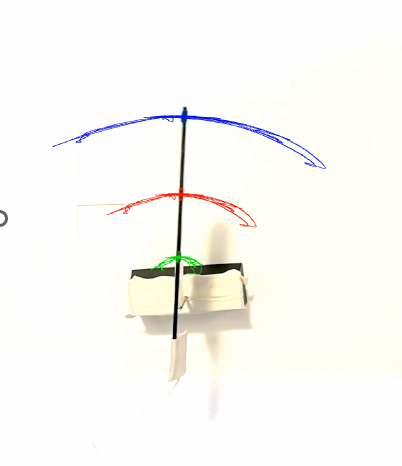
\includegraphics[height = 6.5cm]{figures/MATLAB Generated Wing Tracking Overlay.png}

    \caption{MATLAB Motion Marker Tracking}

    \label{fig:tracking_overlay}

\end{figure}
 
This pipeline now provides deflection histories, calibrated displacement values, trajectories, phase relationships, and spanwise bending shapes, forming the foundation for dynamic comparison between wing geometries. The code was written in a modular way so new wing designs, marker layouts, or additional metrics can be added without rewriting the entire pipeline.
 
\subsection{Preliminary Dynamic Results}

To test the system, several videos were recorded using manually induced flapping. Although the motion was not perfectly smooth or repeatable, it was still useful for checking how well the tracking worked. The tracking was able to follow all three markers throughout the test.

The vertical displacement measured at the root, mid span, and tip is shown in Figure~\ref{fig:tracking_overlay}. The results matched what would be expected for a flexible membrane wing. The tip experienced the largest deflection, the mid span produced a smoother and smaller response, and the root moved only slightly. This behaviour is consistent with bending patterns described in flexible wing literature, such as Shyy et al.~\cite{Shyy2013}.
 
\begin{figure}[htb]

    \centering

    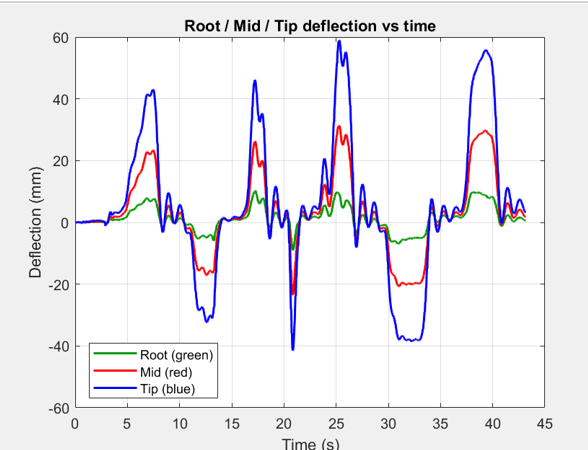
\includegraphics[height = 6.5cm]{figures/Preliminary Wing Deflection.png}

    \caption{Preliminary Vertical Deflection for Manual Flapping}

    \label{fig:dyn_deflection}

\end{figure}
 
In addition to the time based deflection data, I extracted a spanwise deformation shape from the tracked points. This shows the shape of the wing along its span at the moment of maximum tip displacement. The result showed the root nearly stationary, a smooth bending curve through the mid span, and the tip at the largest displacement. This resembles a first mode bending shape and helps compare wings under the same conditions. Being able to extract a mode shape also provides a starting point for linking wing flexibility to aerodynamic behaviour, such as how deformation might influence lift.

 
\begin{figure}[htb]

    \centering

    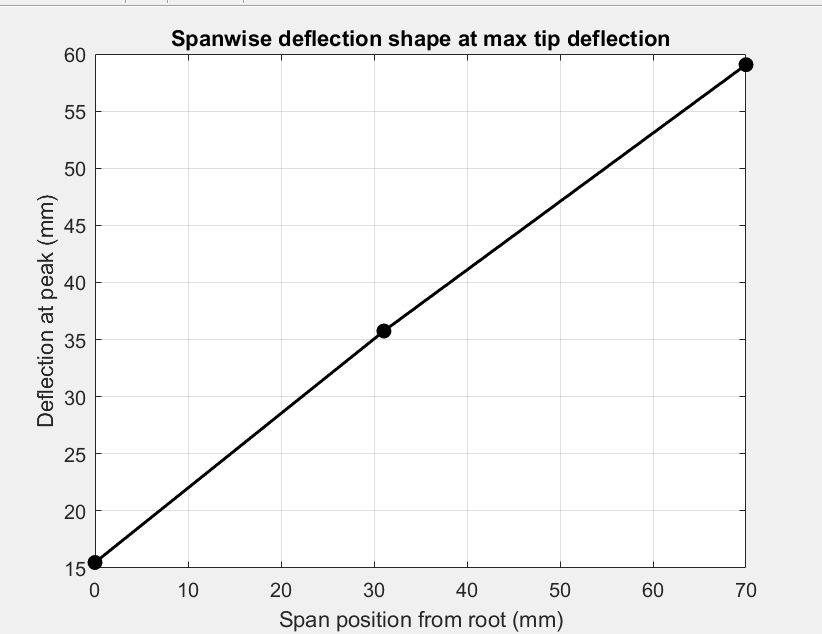
\includegraphics[height = 6.5cm]{figures/Spanwise Deflection Shape.png}

    \caption{Spanwise Deflection - Mode Shape}

    \label{fig:mode_shape}

\end{figure}
 
These results show that the motion tracking system works consistently and that most irregularities came from the manual flapping, not the algorithm. Cleaner and more repeatable data is expected once a motor based flapping system is introduced. Once the servo-driven flapping mechanism is implemented, additional metrics such as dominant flapping frequency, phase lag, and tip velocity will be incorporated into the testing database.
 
\subsection{Use of Previous Static Testing Data}

At the beginning of the term, the static testing results from the previous capstone year were reviewed. Because the wing geometries tested this semester were identical to those previously evaluated, their static stiffness characteristics remain valid. Repeating those tests would not have produced meaningful new insights. This allowed the focus this semester to remain entirely on developing the dynamic testing and motion-tracking framework. Static testing will resume next semester once new wing designs are fabricated so that static and dynamic properties can be documented consistently across all geometries.
 
\subsection{Plan for Winter Semester}

The primary objective for Winter 2026 is to transition from manual excitation to a fully controlled servo-driven flapping mechanism capable of producing consistent, repeatable motion. This will allow precise measurement of dynamic stiffness, deformation patterns, and frequency response. The wing root will be rigidly mounted to eliminate drift observed during preliminary tests. Once new wing geometries are fabricated, each will undergo both static and dynamic characterization. Key parameters such as peak deflection, dominant frequency, phase lag, and spanwise mode shape will be extracted and compiled into a dynamic testing database parallel to the existing static database.
 
A long-term goal is to investigate whether dynamic deformation data can be used to estimate aerodynamic performance, including approximate lift generation. Metrics such as wingtip velocity, instantaneous curvature, and effective angle of attack may be combined with simplified aerodynamic models to infer lift trends. If successful, the dynamic testing platform will provide both structural and aerodynamic insight, strengthening the wing selection process for the Micro Flapping Wing Flyer.
 